\documentclass[11pt,a4paper]{article}

\usepackage[margin=1in]{geometry}
\usepackage{titlesec}
\usepackage{enumitem}
\usepackage{hyperref}
\usepackage{parskip}
\usepackage{graphicx}
\usepackage{float}
\usepackage{booktabs}
\usepackage{amsmath}

\hypersetup{colorlinks=true, linkcolor=blue, urlcolor=blue}

\titleformat{\section}{\large\bfseries}{\thesection}{0.5em}{}
\titleformat{\subsection}{\normalsize\bfseries}{\thesubsection}{0.5em}{}
\setlist{leftmargin=1.4em, topsep=2pt, itemsep=2pt}

\title{\vspace{-1.5cm}\textbf{PKCERT AI \& Software Development Internship \\ Task 12: Clustering \& Dimensionality Reduction}}
\author{Abdullah Amir}
\date{AI and Software Development \\ 17 July 2026}

\begin{document}

\maketitle
\vspace{-0.8cm}

This report covers the theory and the results. The full code, outputs and plots live in
the notebook \texttt{clustering\_dimred.ipynb}. The dataset is \textbf{UCI's Anuran Calls
(MFCCs)}: 7,195 frog call syllables recorded in the field, each described by 22 audio
features, from frogs belonging to a real \textbf{taxonomy} of 4 families, 8 genera and 10
species. That nested taxonomy is why I picked it: it gives the dendrogram in Part B
something real to be judged against, rather than being a decoration.

This is the first \textbf{unsupervised} task, so one ground rule matters throughout. The
taxonomic labels are \emph{never} shown to any model. They are held back entirely and
used only afterwards to score how much of the real structure the clustering recovered.
The results turned out to be full of surprises, most of them the kind that only show up
if you check rather than assume.

% ----------------------------------------------------------------
\section*{Part A: Dataset Selection \& Preparation}

\textbf{What the features are.} Each row is a single \textbf{syllable} of a frog call.
The 22 features are \textbf{MFCCs} (Mel-Frequency Cepstral Coefficients), the standard
way to describe the timbre of a sound. You take the short-term spectrum of the audio,
warp it onto the mel scale (which approximates how ears actually perceive pitch), and
compress the result into a handful of coefficients. The low coefficients capture the
broad shape of the spectrum and the higher ones the finer detail. They are the same
features that underpin speech recognition.

\textbf{Why it suits clustering.} Different species make audibly different calls, so we
would expect the syllables to fall into natural groups without anyone telling the
algorithm what a species is. That is exactly the question clustering asks.

\textbf{Missing values and scaling.} There are no missing values, so nothing needs
imputing. Scaling is more interesting than it first appears. The MFCCs already sit inside
$[-1, 1]$, which tempts you to skip standardising, but their per-feature standard
deviations still differ by roughly fourfold. Every method used here, K-Means, Ward
linkage and PCA, is driven by \textbf{variance and Euclidean distance}, so leaving them
unscaled would let a few high-variance coefficients quietly dominate the distances, the
merges and the principal components alike. I standardised to mean 0 and standard
deviation 1. I also checked for zero-variance columns, which would break the scaler;
there are none.

\textbf{Two caveats that shape everything.} Both are worth stating before any results.

\begin{itemize}
    \item \textbf{The classes are badly imbalanced.} \texttt{AdenomeraHylaedactylus}
    alone accounts for 3,478 of the 7,195 syllables, about 48 percent, while
    \texttt{Rhinellagranulosa} has just 68, under 1 percent. Clustering algorithms chase
    density, so a class that is half the data can easily be split across several
    clusters while rare ones are swallowed whole. That is not a hypothetical: it is
    exactly what happens in Part B.
    \item \textbf{The syllables are not independent.} They come from only \textbf{60
    recordings}, and a single recording contributed 458 syllables. Syllables from one
    recording are the same individual frog, in one place, at one moment, so they are far
    more alike than two random members of a species would be. Any cluster we find may
    partly reflect \emph{a recording} rather than \emph{a species}. No algorithm can fix
    this; it is a property of the data, and it means every score in this report is
    probably optimistic.
\end{itemize}

\begin{figure}[H]
    \centering
    
\includegraphics[width=0.95\textwidth]{figures/01_dataset_overview.png}
    \caption{Left: syllables per species, showing the severe imbalance that drives much
    of what follows. Right: the 22 MFCC features, already bounded in $[-1, 1]$ but with
    visibly different spreads, which is why standardising still matters.}
\end{figure}

% ----------------------------------------------------------------
\section*{Part B: Clustering Techniques}

\subsection*{B1. K-Means and the choice of k}

K-Means picks $k$ centres, assigns each point to the nearest one, moves every centre to
the mean of its members, and repeats until nothing moves. It is fast and simple, but it
carries a strong built-in assumption: that clusters are \textbf{round, similarly sized
blobs}. That assumption turns out to be the whole story of this part.

To choose $k$ I used the two standard tools. The \textbf{elbow method} plots inertia, the
total squared distance from points to their centre, against $k$, looking for a knee where
improvement flattens. The \textbf{silhouette score} measures, for each point, how close
it sits to its own cluster versus the nearest other one, on a scale from $-1$ to $+1$.
Unlike inertia, it does not automatically improve as $k$ grows.

\begin{figure}[H]
    \centering
    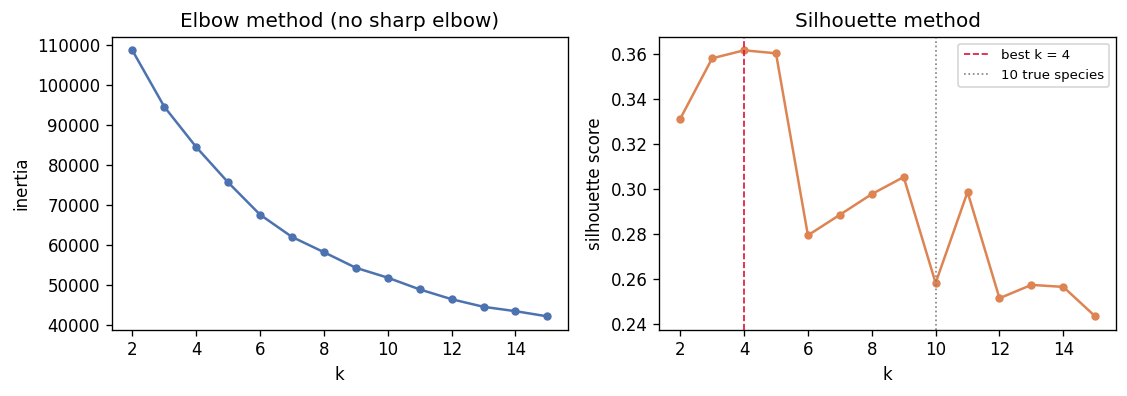
\includegraphics[width=0.85\textwidth]{figures/02_choosing_k.png}
    \caption{Left: the elbow curve bends smoothly with no sharp knee, which is the normal
    case with real data and the reason the elbow method alone is a weak tool. Right: the
    silhouette peaks decisively at k = 4, nowhere near the 10 true species.}
\end{figure}

\textbf{The elbow is a disappointment, and that is worth saying plainly.} There is no
sharp knee to point at; the curve just bends. The silhouette is far more decisive and
peaks at \textbf{k = 4} with a score of 0.362. So the two methods meant to answer ``how
many clusters are there'' suggest \textbf{4}, when we happen to know the truth is
\textbf{10 species}. That disagreement is a genuine finding rather than a bug.

To evaluate the clusters I brought the held-back labels in, using the \textbf{Adjusted
Rand Index (ARI)}, which asks whether the same pairs of points end up together in our
clusters as in the truth, adjusted so that random guessing scores 0, and
\textbf{Normalized Mutual Information (NMI)}, which asks how much knowing the cluster
tells you about the species.

\begin{table}[H]
\centering
\begin{tabular}{lrrr}
\toprule
\textbf{K-Means} & \textbf{ARI vs Family} & \textbf{ARI vs Genus} & \textbf{ARI vs Species} \\
\midrule
k = 4  & 0.446 & 0.502 & \textbf{0.714} \\
k = 8  & 0.284 & 0.342 & 0.524 \\
k = 10 & 0.216 & 0.257 & 0.409 \\
\bottomrule
\end{tabular}
\caption{K-Means scored against all three taxonomic levels.}
\end{table}

Two results here are genuinely surprising, and both survive checking.

\textbf{First, k = 4 does not mean it found the four families.} That is the obvious guess
and it is simply wrong: at k = 4 the ARI against Family is only \textbf{0.446},
\emph{lower} than the same clustering scored against Species (\textbf{0.714}). The four
clusters K-Means likes are not the four families. It would have been very easy to assert
otherwise and never check.

\textbf{Second, k = 4 scores far better against the ten species than k = 10 does}, 0.714
against 0.409. That sounds impossible until you recall what ARI actually penalises:
\emph{splitting} a true group across clusters counts against you just as much as merging
two groups. The dominant species is 48 percent of the data, and at k = 10 K-Means spends
its extra centres carving that one dense blob into pieces rather than isolating the rare
species. The crosstab in the notebook makes this concrete: \texttt{AdenomeraHylaedactylus}
is split across clusters 2, 5 and 8, roughly 1113, 1517 and 834 syllables. K-Means burned
three of its ten clusters on a single species while several rare species got none.

\subsection*{B2. Hierarchical Clustering}

Hierarchical clustering works from the opposite direction. Every point starts as its own
cluster, and the two closest are repeatedly \textbf{merged} until only one remains, with
the entire merge history recorded as a tree. I used \textbf{Ward linkage}, which at each
step merges the pair that increases within-cluster variance the least. Two things make it
attractive here: you do not have to commit to $k$ in advance, since you cut the tree
afterwards wherever you like, and you get nested structure, which is precisely what frog
taxonomy is.

\begin{figure}[H]
    \centering
    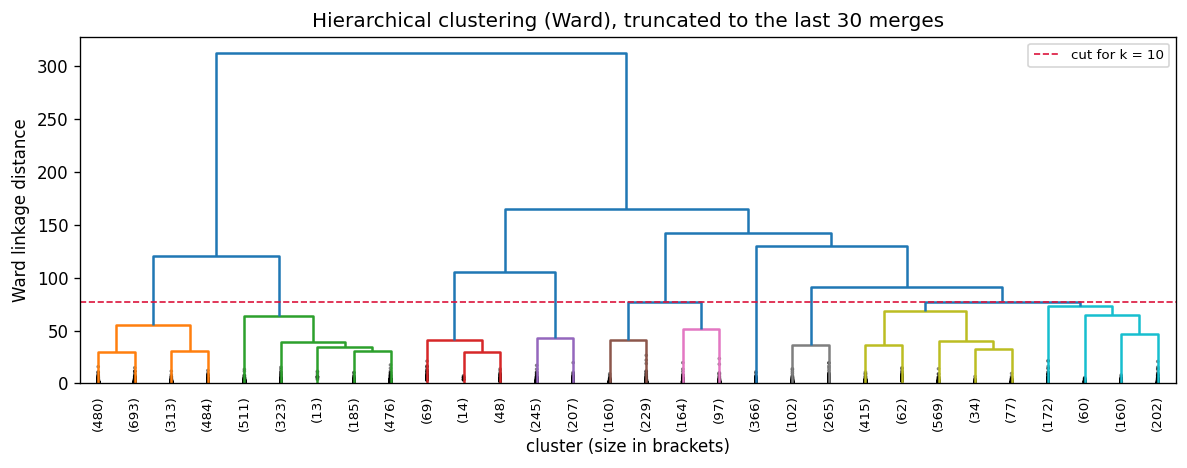
\includegraphics[width=0.88\textwidth]{figures/03_dendrogram.png}
    \caption{The Ward dendrogram. Height is the distance between merged clusters, so tall
    vertical lines mean genuinely distinct groups. With 7,195 leaves the full tree is an
    unreadable smear, so it is truncated to the last 30 merges, each leaf being a whole
    cluster with its size in brackets. The dashed line is the cut giving k = 10.}
\end{figure}

\subsection*{B3. Comparing the two}

\begin{table}[H]
\centering
\begin{tabular}{lrrr}
\toprule
\textbf{Method (k = 10)} & \textbf{ARI vs species} & \textbf{NMI vs species} & \textbf{Silhouette} \\
\midrule
K-Means & 0.409 & 0.613 & 0.258 \\
Ward    & \textbf{0.590} & \textbf{0.719} & \textbf{0.285} \\
\bottomrule
\end{tabular}
\caption{Ward wins on every measure, and the ARI margin is large.}
\end{table}

\textbf{Ward beats K-Means on all three measures}, and the ARI gap (0.590 against 0.409)
is substantial. The reason is the assumption flagged earlier. K-Means insists on round,
roughly equal-sized clusters. This data offers neither: one species has 3,478 syllables
and another has 68, and there is no reason a species' calls should occupy a sphere in
MFCC space. Ward makes no such demand, so it can grow one large cluster alongside several
tiny ones, which is the actual shape of the data. The practical lesson is that K-Means is
not a worse algorithm in general, it just encodes an assumption this dataset violates.

The two methods agree with each other at ARI \textbf{0.554}, which is about as much as
either agrees with the truth. They are finding the same coarse structure and differing on
detail, which is reassuring: there really is signal here and neither is hallucinating.

% ----------------------------------------------------------------
\section*{Part C: Dimensionality Reduction}

\subsection*{C1. PCA}

\textbf{PCA} is \textbf{linear}. It finds the directions of greatest variance and
re-expresses the data along them, in order of importance. It is deterministic, fast, and
each component is a plain weighted sum of the original features, which makes the
transformation reversible and interpretable.

\begin{figure}[H]
    \centering
    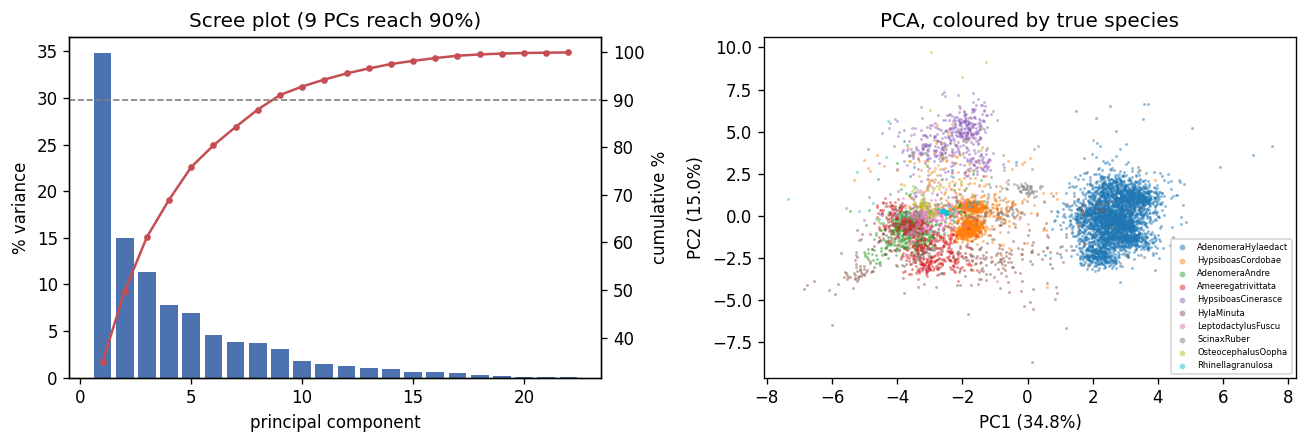
\includegraphics[width=0.95\textwidth]{figures/04_pca.png}
    \caption{Left: the scree plot. PC1 holds 34.8 percent of the variance and PC2 another
    15.0 percent, and it takes 9 components to reach 90 percent. Right: the 2D PCA
    projection coloured by true species, which is honestly a poor picture, with the
    species heavily overlapped.}
\end{figure}

The numbers matter: \textbf{PC1 carries 34.8 percent} and PC2 a further 15.0 percent, so
a 2D PCA plot shows only \textbf{49.8 percent of the variance}. Half the information is
missing from that picture, which is a standing caution against over-reading any 2D
scatter. Reaching 90 percent takes \textbf{9} components and 95 percent takes 12, so the
22 MFCCs are genuinely somewhat redundant but are not compressible to two dimensions
without real loss.

\textbf{Where PCA actually earns its keep} is not as a picture but as a preprocessing
step. Clustering in the 9-component space that holds 90 percent of the variance gives:

\begin{table}[H]
\centering
\begin{tabular}{lr}
\toprule
\textbf{K-Means (k = 10) run on} & \textbf{ARI vs species} \\
\midrule
All 22 scaled features & 0.409 \\
The first 9 principal components & \textbf{0.557} \\
The 2D PCA projection & 0.378 \\
The 2D t-SNE embedding & 0.335 \\
\bottomrule
\end{tabular}
\caption{Dropping 13 of 22 dimensions improved the clustering substantially.}
\end{table}

\textbf{Throwing away 13 of the 22 dimensions made the clustering better}, from ARI 0.409
to \textbf{0.557}. This is not a paradox. The discarded components were mostly noise, and
in a distance-based method, noise spread across 13 directions blurs every distance you
compute. Removing it sharpens the real structure. This ``denoise, then cluster'' pattern
is the strongest practical argument for PCA, and a far better one than any scatter plot.

\subsection*{C2. t-SNE}

\textbf{t-SNE} is \textbf{non-linear} with a completely different goal. It makes no
attempt to preserve variance or global geometry. Instead it measures which points are
\emph{neighbours} in the original 22-dimensional space and arranges points in 2D so those
neighbourhood relationships survive. It exists for looking at data.

\begin{figure}[H]
    \centering
    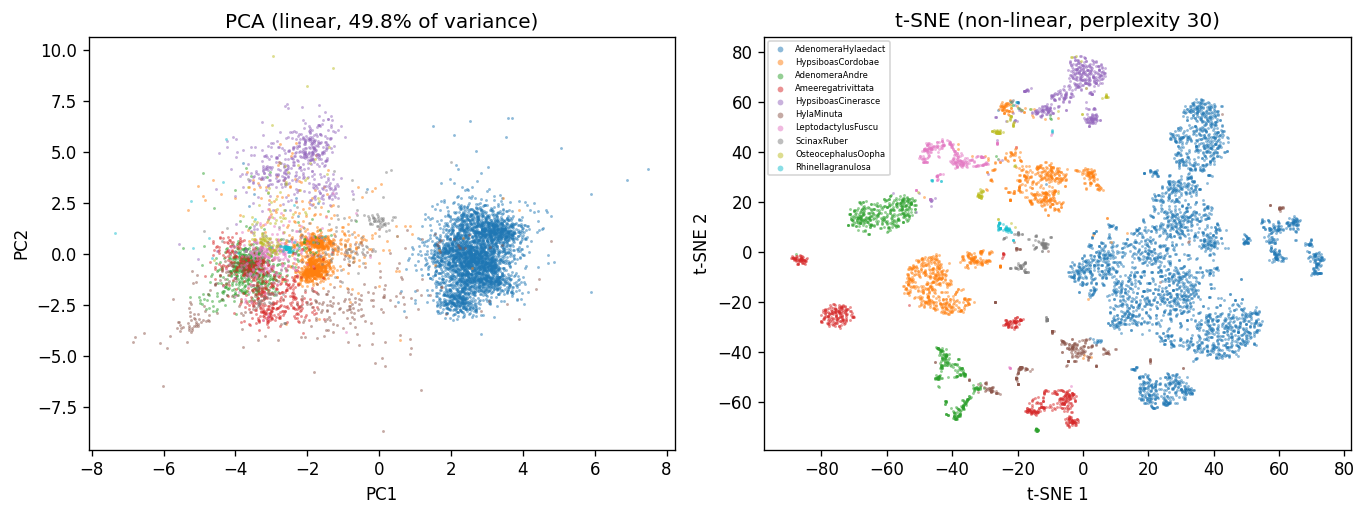
\includegraphics[width=0.95\textwidth]{figures/05_pca_vs_tsne.png}
    \caption{The same data, same colours. PCA (left) smears the species into one
    overlapping cloud. t-SNE (right) resolves them into clearly separated islands that
    align closely with real species. As a picture, t-SNE wins outright.}
\end{figure}

\begin{figure}[H]
    \centering
    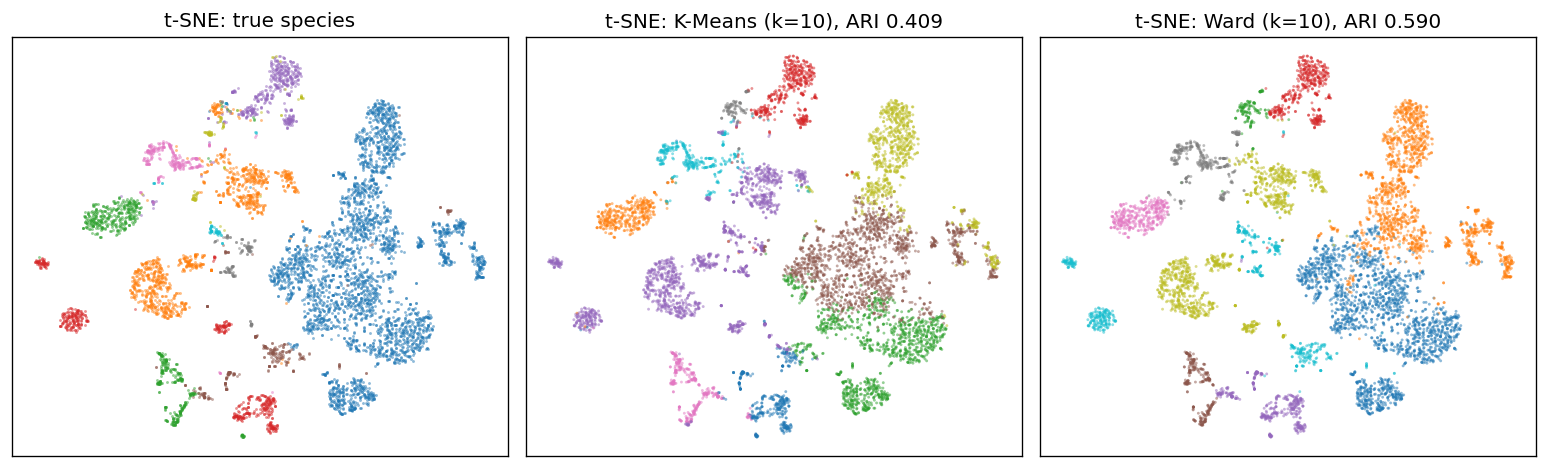
\includegraphics[width=0.95\textwidth]{figures/06_clusters_on_tsne.png}
    \caption{The t-SNE map coloured three ways: by true species, by the K-Means labels,
    and by the Ward labels. Ward's clusters visibly track the real islands more closely
    than K-Means', which is the ARI gap made visual.}
\end{figure}

And now the most important result in this part. \textbf{Clustering on the t-SNE embedding
is the worst option of the four, at ARI 0.335.} The plot that looks the most convincing
produces the weakest clusters, and it is an easy trap to fall into.

The reason is that t-SNE's distances are not real distances. It deliberately distorts
space to make neighbourhoods visible: it inflates dense regions, compresses sparse ones,
and the gaps between its islands carry no information about how different those groups
truly are. K-Means then takes those fictional distances entirely at face value. A t-SNE
plot is a visualisation, not a feature space.

\subsection*{C3. PCA against t-SNE}

\begin{table}[H]
\centering
\begin{tabular}{lll}
\toprule
 & \textbf{PCA} & \textbf{t-SNE} \\
\midrule
Type & Linear projection & Non-linear embedding \\
Preserves & Global structure, variance & Local neighbourhoods \\
Deterministic & Yes & No, varies with the seed \\
Distances meaningful & Yes & \textbf{No} \\
Speed here & Instant & About a minute \\
Handles new data & Yes, just project it & No, must re-run from scratch \\
Interpretable axes & Yes, weighted sums & No, axes mean nothing \\
ARI when clustered on & \textbf{0.557} (9 PCs) & 0.335 \\
\bottomrule
\end{tabular}
\caption{The two methods answer different questions and should not be treated as rivals.}
\end{table}

\textbf{PCA's advantages} are that it is fast, deterministic, reversible, interpretable,
can transform unseen data, and its axes carry a real quantity in variance explained. Its
\textbf{limitation} is that being linear it can only rotate and project, so it cannot
unfold curved structure, which is visible here in that poor 2D picture at 49.8 percent of
variance. \textbf{Use it for} compression, denoising ahead of another algorithm, and
anywhere you must apply the same transform to future data.

\textbf{t-SNE's advantage} is simply that it is a far better picture, revealing structure
PCA smears away. Its \textbf{limitations} are that it is slow, stochastic, sensitive to
the perplexity setting, cannot project new points, and produces distances and gaps that
are not meaningful. \textbf{Use it for} exploring and presenting, and for checking
whether structure exists at all, never as a feature space to compute on.

% ----------------------------------------------------------------
\section*{Part D: Analysis \& Conclusion}

\textbf{What the results say.} Four findings, in order of how much they surprised me.

\begin{enumerate}
    \item \textbf{The data has real structure, but not the ten neat groups you would
    expect.} Every method found genuine signal, with Ward reaching ARI 0.590 against
    species, far above chance. But nothing recovered the ten species cleanly, and the
    silhouette's preferred k = 4 matches neither the 4 families nor the 10 species. The
    honest reading is that frog calls form a handful of strongly separated acoustic
    groups, with finer species distinctions inside them that are much subtler than the
    gaps between groups.
    \item \textbf{Ward beat K-Means because of an assumption, not an accident.} K-Means
    needs round, similar-sized clusters; this data has one species at 48 percent and
    another under 1 percent. Ward requires neither and won on ARI, NMI and silhouette.
    \item \textbf{Fewer dimensions clustered better than more.} K-Means on 9 PCs (0.557)
    clearly beat K-Means on all 22 features (0.409), because the dropped components were
    mostly noise blurring the distances.
    \item \textbf{The best-looking projection made the worst clusters.} t-SNE produced by
    far the most convincing picture and the lowest ARI of any option at 0.335.
\end{enumerate}

\textbf{Recommendation.} \emph{For clustering this dataset, use Hierarchical clustering
with Ward linkage on the first 9 principal components.} Ward is right because it does not
assume spherical, balanced clusters and this data is emphatically neither. Reducing to 9
components first is worth it because that denoising measurably improved K-Means and
should help Ward for the same reason, and it makes the distance computation cheaper.
Ward also spares you committing to $k$ up front, which matters a great deal here given
that none of the methods for choosing $k$ agreed with each other or with the truth.

\emph{For visualising this dataset, use t-SNE, but only for visualising.} It is the only
method that makes the structure legible. Use it to look and to present, then return to
the real feature space, or a PCA of it, to actually compute. \emph{PCA earns its place in
the middle}, not as the visualisation, where at 49.8 percent of variance in 2D it is
honestly poor, but as the preprocessing step that made the clustering better.

\textbf{The caveat that matters most.} Every score in this report is probably
\emph{optimistic}, and it would be dishonest to present them without saying so. The 7,195
syllables come from only 60 recordings, so syllables from one recording are the same
individual frog in a single moment, and are far more alike than two random members of a
species would be. Some of what these clusters ``discovered'' is almost certainly
\emph{this particular frog on this particular evening} rather than \emph{this species}. A
stricter evaluation would group syllables by \texttt{RecordID} and test whether clusters
survive across different recordings of the same species. With only 3 to 11 recordings per
species that test would be underpowered, which is a limitation of the dataset rather than
of the methods, but it is the first thing I would want more data for.

\textbf{Conclusion.} The thread running through this whole task is that unsupervised
learning gives you no accuracy score to hide behind. The elbow method gave no answer, the
silhouette gave a confident answer that was wrong, the intuitive guess that k = 4 meant
``the four families'' was false when checked, the prettiest plot was the least
trustworthy, and throwing away half the dimensions improved the result. Not one of those
would have been caught by looking at a single number. When there is no ground truth to
appeal to, and in a real clustering problem there is none, reading the results sceptically
is not an optional extra: it is the entire job.

\vspace{0.4cm}
The notebook and README are on GitHub:
\url{https://github.com/AbdullahAmir06/ai-internship-abdullahamir}.

\end{document}
